\documentclass{book}
\usepackage[a4paper,top=2.5cm,bottom=2.5cm,left=2.5cm,right=2.5cm]{geometry}
\usepackage{makeidx}
\usepackage{natbib}
\usepackage{graphicx}
\usepackage{multicol}
\usepackage{float}
\usepackage{listings}
\usepackage{color}
\usepackage{ifthen}
\usepackage[table]{xcolor}
\usepackage{textcomp}
\usepackage{alltt}
\usepackage{ifpdf}
\ifpdf
\usepackage[pdftex,
            pagebackref=true,
            colorlinks=true,
            linkcolor=blue,
            unicode
           ]{hyperref}
\else
\usepackage[ps2pdf,
            pagebackref=true,
            colorlinks=true,
            linkcolor=blue,
            unicode
           ]{hyperref}
\usepackage{pspicture}
\fi
\usepackage[utf8]{inputenc}
\usepackage{mathptmx}
\usepackage[scaled=.90]{helvet}
\usepackage{courier}
\usepackage{sectsty}
\usepackage{amssymb}
\usepackage[titles]{tocloft}
\usepackage{doxygen}
\lstset{language=C++,inputencoding=utf8,basicstyle=\footnotesize,breaklines=true,breakatwhitespace=true,tabsize=4,numbers=left }
\makeindex
\setcounter{tocdepth}{3}
\renewcommand{\footrulewidth}{0.4pt}
\renewcommand{\familydefault}{\sfdefault}
\hfuzz=15pt
\setlength{\emergencystretch}{15pt}
\hbadness=750
\tolerance=750
\begin{document}
\hypersetup{pageanchor=false,citecolor=blue}
\begin{titlepage}
\vspace*{7cm}
\begin{center}
{\Large Un\-Banco \\[1ex]\large 1.\-0 }\\
\vspace*{1cm}
{\large Generated by Doxygen 1.8.3.1}\\
\vspace*{0.5cm}
{\small Wed May 15 2013 11:00:24}\\
\end{center}
\end{titlepage}
\clearemptydoublepage
\pagenumbering{roman}
\tableofcontents
\clearemptydoublepage
\pagenumbering{arabic}
\hypersetup{pageanchor=true,citecolor=blue}
\chapter{Hierarchical Index}
\section{Class Hierarchy}
This inheritance list is sorted roughly, but not completely, alphabetically\-:\begin{DoxyCompactList}
\item \contentsline{section}{Account}{\pageref{d7/d10/classAccount}}{}
\item \contentsline{section}{Main\-Interface}{\pageref{d2/da2/classMainInterface}}{}
\begin{DoxyCompactList}
\item \contentsline{section}{Main\-Adm\-Menu}{\pageref{d9/d86/classMainAdmMenu}}{}
\item \contentsline{section}{Main\-Cus\-Menu}{\pageref{dc/d35/classMainCusMenu}}{}
\item \contentsline{section}{Main\-Login}{\pageref{db/df3/classMainLogin}}{}
\item \contentsline{section}{Main\-Man\-Menu}{\pageref{d0/d1d/classMainManMenu}}{}
\end{DoxyCompactList}
\item \contentsline{section}{Payment}{\pageref{d5/d5e/classPayment}}{}
\item \contentsline{section}{Pers\-Error}{\pageref{da/dcf/classPersError}}{}
\item \contentsline{section}{Test$<$ info\-Type, class\-Type $>$}{\pageref{df/da6/classTest}}{}
\item \contentsline{section}{Transac\-Adm}{\pageref{da/deb/classTransacAdm}}{}
\item \contentsline{section}{Unit\-Base$<$ base\-Type $>$}{\pageref{d5/db5/classUnitBase}}{}
\item \contentsline{section}{Unit\-Base$<$ bool $>$}{\pageref{d5/db5/classUnitBase}}{}
\begin{DoxyCompactList}
\item \contentsline{section}{Usr\-Type}{\pageref{d1/dd4/classUsrType}}{}
\end{DoxyCompactList}
\item \contentsline{section}{Unit\-Base$<$ float $>$}{\pageref{d5/db5/classUnitBase}}{}
\begin{DoxyCompactList}
\item \contentsline{section}{Money}{\pageref{d7/d9a/classMoney}}{}
\end{DoxyCompactList}
\item \contentsline{section}{Unit\-Base$<$ int $>$}{\pageref{d5/db5/classUnitBase}}{}
\begin{DoxyCompactList}
\item \contentsline{section}{Acc\-Number}{\pageref{df/d00/classAccNumber}}{}
\item \contentsline{section}{Pay\-Code}{\pageref{d0/d34/classPayCode}}{}
\item \contentsline{section}{Pay\-Day}{\pageref{dc/d17/classPayDay}}{}
\item \contentsline{section}{Usr\-Id}{\pageref{d8/dc7/classUsrId}}{}
\item \contentsline{section}{Usr\-Matric}{\pageref{d4/d69/classUsrMatric}}{}
\end{DoxyCompactList}
\item \contentsline{section}{Unit\-Base$<$ string $>$}{\pageref{d5/db5/classUnitBase}}{}
\begin{DoxyCompactList}
\item \contentsline{section}{Usr\-Name}{\pageref{da/df7/classUsrName}}{}
\item \contentsline{section}{Usr\-Password}{\pageref{d9/d39/classUsrPassword}}{}
\end{DoxyCompactList}
\item \contentsline{section}{User}{\pageref{d9/dc0/classUser}}{}
\begin{DoxyCompactList}
\item \contentsline{section}{Customer}{\pageref{d9/d12/classCustomer}}{}
\item \contentsline{section}{Manager}{\pageref{dd/dcd/classManager}}{}
\end{DoxyCompactList}
\item \contentsline{section}{User\-Adm}{\pageref{de/dac/classUserAdm}}{}
\item \contentsline{section}{User\-Login}{\pageref{d4/de1/classUserLogin}}{}
\begin{DoxyCompactList}
\item \contentsline{section}{Stub}{\pageref{df/d32/classStub}}{}
\end{DoxyCompactList}
\item \contentsline{section}{Window}{\pageref{dc/dc4/classWindow}}{}
\begin{DoxyCompactList}
\item \contentsline{section}{Textual}{\pageref{de/da3/classTextual}}{}
\end{DoxyCompactList}
\end{DoxyCompactList}

\chapter{Class Index}
\section{Class List}
Here are the classes, structs, unions and interfaces with brief descriptions\-:\begin{DoxyCompactList}
\item\contentsline{section}{\hyperlink{classAccNumber}{Acc\-Number} \\*Define o número da conta de um \hyperlink{classCustomer}{Customer} (Cliente) }{\pageref{classAccNumber}}{}
\item\contentsline{section}{\hyperlink{classAccount}{Account} \\*Conta; Onde ficarão armazenados os dados de conta de um cliente }{\pageref{classAccount}}{}
\item\contentsline{section}{\hyperlink{classCustomer}{Customer} \\*Cliente; Onde ficarão armazenados os dados do usuário padrão do sistema }{\pageref{classCustomer}}{}
\item\contentsline{section}{\hyperlink{classManager}{Manager} \\*Gerente; Onde ficarão armazenados os dados de usuários com privilégios administrativos sobre o sistema }{\pageref{classManager}}{}
\item\contentsline{section}{\hyperlink{classMoney}{Money} \\*Define o limite da conta de um \hyperlink{classCustomer}{Customer} (Cliente) }{\pageref{classMoney}}{}
\item\contentsline{section}{\hyperlink{classPayCode}{Pay\-Code} \\*Define um número de identificação para cada pagamento }{\pageref{classPayCode}}{}
\item\contentsline{section}{\hyperlink{classPayDay}{Pay\-Day} \\*Define a data do pagamento }{\pageref{classPayDay}}{}
\item\contentsline{section}{\hyperlink{classPayment}{Payment} \\*Pagamento; Onde ficarão armazenados dados sobre pagamentos a serem realizados }{\pageref{classPayment}}{}
\item\contentsline{section}{\hyperlink{classTest}{Test$<$ info\-Type, class\-Type $>$} }{\pageref{classTest}}{}
\item\contentsline{section}{\hyperlink{classUnitBase}{Unit\-Base$<$ base\-Type $>$} \\*A base de derivação de todas as classes de tipos básicos }{\pageref{classUnitBase}}{}
\item\contentsline{section}{\hyperlink{classUser}{User} \\*Usuário; Base de derivação das classes \hyperlink{classCustomer}{Customer} e \hyperlink{classManager}{Manager} }{\pageref{classUser}}{}
\item\contentsline{section}{\hyperlink{classUsrId}{Usr\-Id} \\*Define o I\-D de um \hyperlink{classCustomer}{Customer} }{\pageref{classUsrId}}{}
\item\contentsline{section}{\hyperlink{classUsrMatric}{Usr\-Matric} \\*Define a matrícula de um \hyperlink{classManager}{Manager} }{\pageref{classUsrMatric}}{}
\item\contentsline{section}{\hyperlink{classUsrName}{Usr\-Name} \\*Define o nome de um \hyperlink{classUser}{User} (\hyperlink{classCustomer}{Customer} ou \hyperlink{classManager}{Manager}) }{\pageref{classUsrName}}{}
\item\contentsline{section}{\hyperlink{classUsrPassword}{Usr\-Password} \\*Define a senha de um \hyperlink{classUser}{User} (\hyperlink{classCustomer}{Customer} ou \hyperlink{classManager}{Manager}) }{\pageref{classUsrPassword}}{}
\item\contentsline{section}{\hyperlink{classUsrType}{Usr\-Type} \\*Codifica tipos de conta }{\pageref{classUsrType}}{}
\end{DoxyCompactList}

\chapter{Class Documentation}
\hypertarget{classAccNumber}{\section{Acc\-Number Class Reference}
\label{classAccNumber}\index{Acc\-Number@{Acc\-Number}}
}


Define o número da conta de um Customer (Cliente).  




{\ttfamily \#include $<$Base\-Unit.\-h$>$}

Inheritance diagram for Acc\-Number\-:\begin{figure}[H]
\begin{center}
\leavevmode
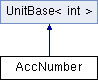
\includegraphics[height=2.000000cm]{classAccNumber}
\end{center}
\end{figure}
\subsection*{Public Member Functions}
\begin{DoxyCompactItemize}
\item 
\hypertarget{classAccNumber_a11a8a2ea0849a83365960758a5ff3362}{{\bfseries Acc\-Number} (int)  throw (invalid\-\_\-argument)}\label{classAccNumber_a11a8a2ea0849a83365960758a5ff3362}

\end{DoxyCompactItemize}
\subsection*{Additional Inherited Members}


\subsection{Detailed Description}
Define o número da conta de um Customer (Cliente). 

Este tipo básico tem a função de atribuir a cada conta um numero unico, identificando-\/a. 

The documentation for this class was generated from the following files\-:\begin{DoxyCompactItemize}
\item 
Base\-Unit.\-h\item 
Base\-Unit.\-cpp\end{DoxyCompactItemize}

\hypertarget{classMoney}{\section{Money Class Reference}
\label{classMoney}\index{Money@{Money}}
}


Define o limite da conta de um \hyperlink{classCustomer}{Customer} (Cliente).  




{\ttfamily \#include $<$Base\-Unit.\-h$>$}

Inheritance diagram for Money\-:\begin{figure}[H]
\begin{center}
\leavevmode
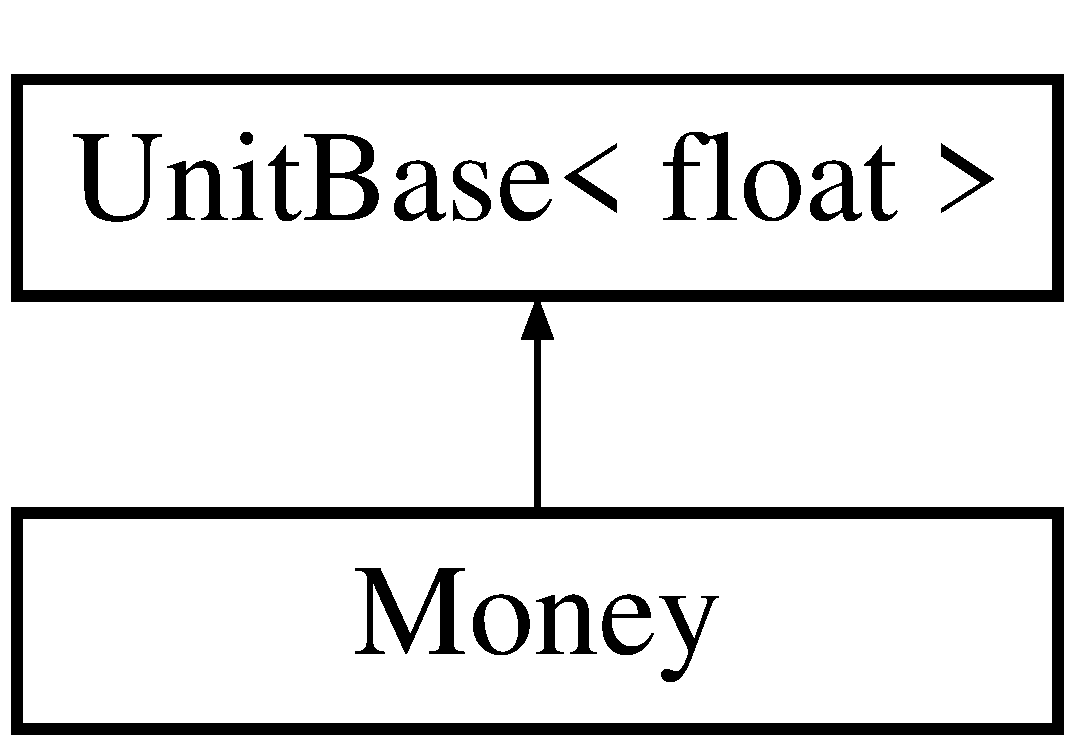
\includegraphics[height=2.000000cm]{classMoney}
\end{center}
\end{figure}
\subsection*{Public Member Functions}
\begin{DoxyCompactItemize}
\item 
\hypertarget{classMoney_a33986736e7432883ebd61584815b6681}{{\bfseries Money} (const float \&)  throw (invalid\-\_\-argument)}\label{classMoney_a33986736e7432883ebd61584815b6681}

\end{DoxyCompactItemize}
\subsection*{Additional Inherited Members}


\subsection{Detailed Description}
Define o limite da conta de um \hyperlink{classCustomer}{Customer} (Cliente). 

Atribui a cada conta um limite, limitando a utilização do crédito junto ao banco. 

The documentation for this class was generated from the following files\-:\begin{DoxyCompactItemize}
\item 
Base\-Unit.\-h\item 
Base\-Unit.\-cpp\end{DoxyCompactItemize}

\hypertarget{classPayCode}{\section{Pay\-Code Class Reference}
\label{classPayCode}\index{Pay\-Code@{Pay\-Code}}
}


Define um número de identificação para cada pagamento.  




{\ttfamily \#include $<$Base\-Unit.\-h$>$}

Inheritance diagram for Pay\-Code\-:\begin{figure}[H]
\begin{center}
\leavevmode
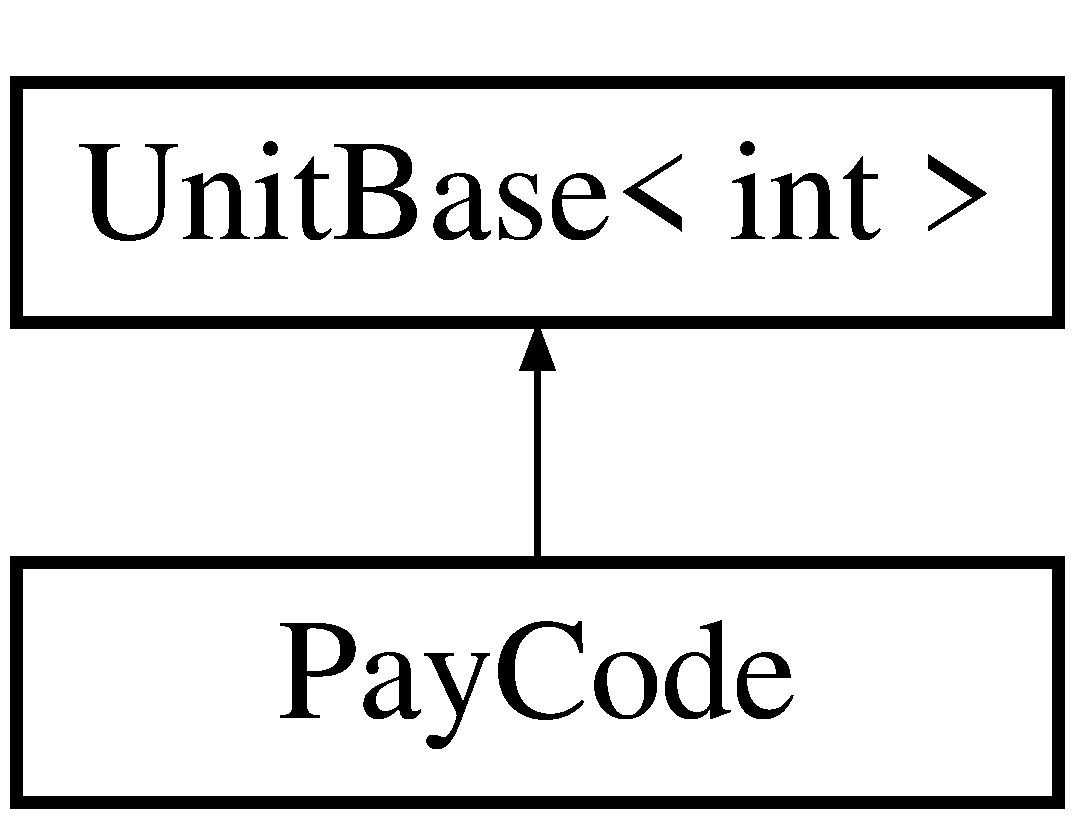
\includegraphics[height=2.000000cm]{classPayCode}
\end{center}
\end{figure}
\subsection*{Public Member Functions}
\begin{DoxyCompactItemize}
\item 
\hypertarget{classPayCode_a919ab6e420b9bd55e8c470ea411aa97e}{{\bfseries Pay\-Code} (const int \&)  throw (invalid\-\_\-argument)}\label{classPayCode_a919ab6e420b9bd55e8c470ea411aa97e}

\end{DoxyCompactItemize}
\subsection*{Additional Inherited Members}


\subsection{Detailed Description}
Define um número de identificação para cada pagamento. 

Atribui a cada pagamento um código, de forma a identificá-\/lo. 

The documentation for this class was generated from the following files\-:\begin{DoxyCompactItemize}
\item 
Base\-Unit.\-h\item 
Base\-Unit.\-cpp\end{DoxyCompactItemize}

\hypertarget{classPayDay}{\subsection{Pay\-Day Class Reference}
\label{dc/d17/classPayDay}\index{Pay\-Day@{Pay\-Day}}
}


Define a data do pagamento.  




{\ttfamily \#include $<$Base\-Unit.\-h$>$}

Inheritance diagram for Pay\-Day\-:\begin{figure}[H]
\begin{center}
\leavevmode
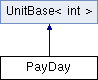
\includegraphics[height=2.000000cm]{dc/d17/classPayDay}
\end{center}
\end{figure}
\subsubsection*{Public Member Functions}
\begin{DoxyCompactItemize}
\item 
\hyperlink{classPayDay_a6da36cea0b2ac9a53106552aad00996a}{Pay\-Day} ()
\begin{DoxyCompactList}\small\item\em Construtor padrão de \hyperlink{classPayDay}{Pay\-Day}. \end{DoxyCompactList}\item 
\hyperlink{classPayDay_aa11abdfdb58bbd93f68bc02a7496e1c4}{Pay\-Day} (const int \&)  throw (invalid\-\_\-argument)
\begin{DoxyCompactList}\small\item\em Construtor base de \hyperlink{classPayDay}{Pay\-Day}. \end{DoxyCompactList}\item 
int \hyperlink{classPayDay_a297ce892f49aa9f3a504d514f171ed1d}{day} ()
\begin{DoxyCompactList}\small\item\em Método que retorna o dia contido na data. \end{DoxyCompactList}\item 
int \hyperlink{classPayDay_ada65e8834c142a95cd35ca2b399fbcde}{month} ()
\begin{DoxyCompactList}\small\item\em Método que retorna o mês contido na data. \end{DoxyCompactList}\item 
int \hyperlink{classPayDay_a962960925f9e6eaaac0fef5eb96849ec}{year} ()
\begin{DoxyCompactList}\small\item\em Método que retorna o ano contido na data. \end{DoxyCompactList}\end{DoxyCompactItemize}
\subsubsection*{Additional Inherited Members}


\subsubsection{Detailed Description}
Define a data do pagamento. 

Guarda a data de um pagamento num inteiro de formato D\-D\-M\-M\-A\-A\-A\-A. Dia, mês e ano devem ser acessados através dos atributos day, month, year. 

Definition at line 196 of file Base\-Unit.\-h.



\subsubsection{Constructor \& Destructor Documentation}
\hypertarget{classPayDay_a6da36cea0b2ac9a53106552aad00996a}{\index{Pay\-Day@{Pay\-Day}!Pay\-Day@{Pay\-Day}}
\index{Pay\-Day@{Pay\-Day}!PayDay@{Pay\-Day}}
\paragraph[{Pay\-Day}]{\setlength{\rightskip}{0pt plus 5cm}Pay\-Day\-::\-Pay\-Day (
\begin{DoxyParamCaption}
{}
\end{DoxyParamCaption}
)}}\label{dc/d17/classPayDay_a6da36cea0b2ac9a53106552aad00996a}


Construtor padrão de \hyperlink{classPayDay}{Pay\-Day}. 

Define o valor 0 como valor de não-\/inicialização deste tipo básico. 

Definition at line 173 of file Base\-Unit.\-cpp.

\hypertarget{classPayDay_aa11abdfdb58bbd93f68bc02a7496e1c4}{\index{Pay\-Day@{Pay\-Day}!Pay\-Day@{Pay\-Day}}
\index{Pay\-Day@{Pay\-Day}!PayDay@{Pay\-Day}}
\paragraph[{Pay\-Day}]{\setlength{\rightskip}{0pt plus 5cm}Pay\-Day\-::\-Pay\-Day (
\begin{DoxyParamCaption}
\item[{const int \&}]{date}
\end{DoxyParamCaption}
)  throw (invalid\-\_\-argument)}}\label{dc/d17/classPayDay_aa11abdfdb58bbd93f68bc02a7496e1c4}


Construtor base de \hyperlink{classPayDay}{Pay\-Day}. 

É preferível que se utilize este construtor pois ele já faz a validação automática do valor a ser definido. 

Definition at line 178 of file Base\-Unit.\-cpp.



\subsubsection{Member Function Documentation}
\hypertarget{classPayDay_a297ce892f49aa9f3a504d514f171ed1d}{\index{Pay\-Day@{Pay\-Day}!day@{day}}
\index{day@{day}!PayDay@{Pay\-Day}}
\paragraph[{day}]{\setlength{\rightskip}{0pt plus 5cm}int Pay\-Day\-::day (
\begin{DoxyParamCaption}
{}
\end{DoxyParamCaption}
)\hspace{0.3cm}{\ttfamily [inline]}}}\label{dc/d17/classPayDay_a297ce892f49aa9f3a504d514f171ed1d}


Método que retorna o dia contido na data. 

Extrai do inteiro contido no objeto o dia a que ele se refere. 

Definition at line 231 of file Base\-Unit.\-h.

\hypertarget{classPayDay_ada65e8834c142a95cd35ca2b399fbcde}{\index{Pay\-Day@{Pay\-Day}!month@{month}}
\index{month@{month}!PayDay@{Pay\-Day}}
\paragraph[{month}]{\setlength{\rightskip}{0pt plus 5cm}int Pay\-Day\-::month (
\begin{DoxyParamCaption}
{}
\end{DoxyParamCaption}
)\hspace{0.3cm}{\ttfamily [inline]}}}\label{dc/d17/classPayDay_ada65e8834c142a95cd35ca2b399fbcde}


Método que retorna o mês contido na data. 

Extrai do inteiro contido no objeto o mês a que ele se refere. 

Definition at line 226 of file Base\-Unit.\-h.

\hypertarget{classPayDay_a962960925f9e6eaaac0fef5eb96849ec}{\index{Pay\-Day@{Pay\-Day}!year@{year}}
\index{year@{year}!PayDay@{Pay\-Day}}
\paragraph[{year}]{\setlength{\rightskip}{0pt plus 5cm}int Pay\-Day\-::year (
\begin{DoxyParamCaption}
{}
\end{DoxyParamCaption}
)\hspace{0.3cm}{\ttfamily [inline]}}}\label{dc/d17/classPayDay_a962960925f9e6eaaac0fef5eb96849ec}


Método que retorna o ano contido na data. 

Extrai do inteiro contido no objeto o ano a que ele se refere. 

Definition at line 221 of file Base\-Unit.\-h.



The documentation for this class was generated from the following files\-:\begin{DoxyCompactItemize}
\item 
Base\-Unit.\-h\item 
Base\-Unit.\-cpp\end{DoxyCompactItemize}

\hypertarget{classPayValue}{\section{Pay\-Value Class Reference}
\label{classPayValue}\index{Pay\-Value@{Pay\-Value}}
}


Define o valor do pagamento.  




{\ttfamily \#include $<$Base\-Unit.\-h$>$}

Inheritance diagram for Pay\-Value\-:\begin{figure}[H]
\begin{center}
\leavevmode
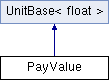
\includegraphics[height=2.000000cm]{classPayValue}
\end{center}
\end{figure}
\subsection*{Public Member Functions}
\begin{DoxyCompactItemize}
\item 
\hypertarget{classPayValue_a94fd7f5521beb8a47dbd34e6e0671a11}{{\bfseries Pay\-Value} (float)  throw (invalid\-\_\-argument)}\label{classPayValue_a94fd7f5521beb8a47dbd34e6e0671a11}

\end{DoxyCompactItemize}
\subsection*{Additional Inherited Members}


\subsection{Detailed Description}
Define o valor do pagamento. 

Recorda o valor de um pagamento. 

The documentation for this class was generated from the following files\-:\begin{DoxyCompactItemize}
\item 
Base\-Unit.\-h\item 
Base\-Unit.\-cpp\end{DoxyCompactItemize}

\hypertarget{classUnitBase}{\section{Unit\-Base$<$ base\-Type $>$ Class Template Reference}
\label{d5/db5/classUnitBase}\index{Unit\-Base$<$ base\-Type $>$@{Unit\-Base$<$ base\-Type $>$}}
}


A base de derivação de todas as classes de tipos básicos.  




{\ttfamily \#include $<$Base\-Unit.\-h$>$}

\subsection*{Public Member Functions}
\begin{DoxyCompactItemize}
\item 
void \hyperlink{classUnitBase_a9cd392786b8078ab713045a8d1dece52}{set\-Value} (base\-Type \hyperlink{classUnitBase_a1c1ad08b45f07a94e5cf71dee734436b}{value})  throw (invalid\-\_\-argument)
\begin{DoxyCompactList}\small\item\em Método que define o valor do atributo value. \end{DoxyCompactList}\item 
base\-Type \hyperlink{classUnitBase_a6b4041c7176acb6c4956e085603449d1}{get\-Value} () const 
\begin{DoxyCompactList}\small\item\em Método que recupera o valor do atributo value. \end{DoxyCompactList}\end{DoxyCompactItemize}
\subsection*{Protected Attributes}
\begin{DoxyCompactItemize}
\item 
base\-Type \hyperlink{classUnitBase_a1c1ad08b45f07a94e5cf71dee734436b}{value}
\begin{DoxyCompactList}\small\item\em O valor comportado pela unidade. \end{DoxyCompactList}\end{DoxyCompactItemize}


\subsection{Detailed Description}
\subsubsection*{template$<$typename base\-Type$>$class Unit\-Base$<$ base\-Type $>$}

A base de derivação de todas as classes de tipos básicos. 

Suas diferentes instâncias servem de base para a construção de todos os outros tipos básicos. 

\subsection{Member Function Documentation}
\hypertarget{classUnitBase_a6b4041c7176acb6c4956e085603449d1}{\index{Unit\-Base@{Unit\-Base}!get\-Value@{get\-Value}}
\index{get\-Value@{get\-Value}!UnitBase@{Unit\-Base}}
\subsubsection[{get\-Value}]{\setlength{\rightskip}{0pt plus 5cm}template$<$typename base\-Type$>$ base\-Type {\bf Unit\-Base}$<$ base\-Type $>$\-::get\-Value (
\begin{DoxyParamCaption}
{}
\end{DoxyParamCaption}
) const\hspace{0.3cm}{\ttfamily [inline]}}}\label{d5/db5/classUnitBase_a6b4041c7176acb6c4956e085603449d1}


Método que recupera o valor do atributo value. 

O valor é retornado por este método, e o atributo não é modificado no processo. \hypertarget{classUnitBase_a9cd392786b8078ab713045a8d1dece52}{\index{Unit\-Base@{Unit\-Base}!set\-Value@{set\-Value}}
\index{set\-Value@{set\-Value}!UnitBase@{Unit\-Base}}
\subsubsection[{set\-Value}]{\setlength{\rightskip}{0pt plus 5cm}template$<$typename base\-Type$>$ void {\bf Unit\-Base}$<$ base\-Type $>$\-::set\-Value (
\begin{DoxyParamCaption}
\item[{base\-Type}]{value}
\end{DoxyParamCaption}
)  throw (invalid\-\_\-argument)\hspace{0.3cm}{\ttfamily [inline]}}}\label{d5/db5/classUnitBase_a9cd392786b8078ab713045a8d1dece52}


Método que define o valor do atributo value. 

A validação ocorre no processo, e o valor não será setado no caso do argumento deste método ser inválido. 

\subsection{Member Data Documentation}
\hypertarget{classUnitBase_a1c1ad08b45f07a94e5cf71dee734436b}{\index{Unit\-Base@{Unit\-Base}!value@{value}}
\index{value@{value}!UnitBase@{Unit\-Base}}
\subsubsection[{value}]{\setlength{\rightskip}{0pt plus 5cm}template$<$typename base\-Type$>$ base\-Type {\bf Unit\-Base}$<$ base\-Type $>$\-::value\hspace{0.3cm}{\ttfamily [protected]}}}\label{d5/db5/classUnitBase_a1c1ad08b45f07a94e5cf71dee734436b}


O valor comportado pela unidade. 

Seu tipo varia de acordo com a forma que o template é instanciado. 

The documentation for this class was generated from the following file\-:\begin{DoxyCompactItemize}
\item 
Base\-Unit.\-h\end{DoxyCompactItemize}

\hypertarget{classUsrId}{\section{Usr\-Id Class Reference}
\label{d8/dc7/classUsrId}\index{Usr\-Id@{Usr\-Id}}
}


Define o I\-D de um \hyperlink{classCustomer}{Customer}.  




{\ttfamily \#include $<$Base\-Unit.\-h$>$}

Inheritance diagram for Usr\-Id\-:\begin{figure}[H]
\begin{center}
\leavevmode
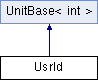
\includegraphics[height=2.000000cm]{d8/dc7/classUsrId}
\end{center}
\end{figure}
\subsection*{Public Member Functions}
\begin{DoxyCompactItemize}
\item 
\hyperlink{classUsrId_a55a05b8f951a218c66c49f09fa6ce374}{Usr\-Id} ()
\begin{DoxyCompactList}\small\item\em Construtor padrão de \hyperlink{classUsrId}{Usr\-Id}. \end{DoxyCompactList}\item 
\hyperlink{classUsrId_a3be81b6f539c0121803f9d88e9d89553}{Usr\-Id} (const int \&)  throw (invalid\-\_\-argument)
\begin{DoxyCompactList}\small\item\em Construtor base de \hyperlink{classUsrId}{Usr\-Id}. \end{DoxyCompactList}\end{DoxyCompactItemize}
\subsection*{Additional Inherited Members}


\subsection{Detailed Description}
Define o I\-D de um \hyperlink{classCustomer}{Customer}. 

Tem a função de identificar de forma única um \hyperlink{classCustomer}{Customer}, independentemente do seu tipo de conta. 

\subsection{Constructor \& Destructor Documentation}
\hypertarget{classUsrId_a55a05b8f951a218c66c49f09fa6ce374}{\index{Usr\-Id@{Usr\-Id}!Usr\-Id@{Usr\-Id}}
\index{Usr\-Id@{Usr\-Id}!UsrId@{Usr\-Id}}
\subsubsection[{Usr\-Id}]{\setlength{\rightskip}{0pt plus 5cm}Usr\-Id\-::\-Usr\-Id (
\begin{DoxyParamCaption}
{}
\end{DoxyParamCaption}
)}}\label{d8/dc7/classUsrId_a55a05b8f951a218c66c49f09fa6ce374}


Construtor padrão de \hyperlink{classUsrId}{Usr\-Id}. 

Define o valor 0 como valor de não-\/inicialização deste tipo básico. \hypertarget{classUsrId_a3be81b6f539c0121803f9d88e9d89553}{\index{Usr\-Id@{Usr\-Id}!Usr\-Id@{Usr\-Id}}
\index{Usr\-Id@{Usr\-Id}!UsrId@{Usr\-Id}}
\subsubsection[{Usr\-Id}]{\setlength{\rightskip}{0pt plus 5cm}Usr\-Id\-::\-Usr\-Id (
\begin{DoxyParamCaption}
\item[{const int \&}]{usr\-Id}
\end{DoxyParamCaption}
)  throw (invalid\-\_\-argument)}}\label{d8/dc7/classUsrId_a3be81b6f539c0121803f9d88e9d89553}


Construtor base de \hyperlink{classUsrId}{Usr\-Id}. 

É preferível que se utilize este construtor, pois ele já faz a validação automática do valor a ser definido. 

The documentation for this class was generated from the following files\-:\begin{DoxyCompactItemize}
\item 
Base\-Unit.\-h\item 
Base\-Unit.\-cpp\end{DoxyCompactItemize}

\hypertarget{classUsrMatric}{\section{Usr\-Matric Class Reference}
\label{classUsrMatric}\index{Usr\-Matric@{Usr\-Matric}}
}


Define a matrícula de um \hyperlink{classManager}{Manager}.  




{\ttfamily \#include $<$Base\-Unit.\-h$>$}

Inheritance diagram for Usr\-Matric\-:\begin{figure}[H]
\begin{center}
\leavevmode
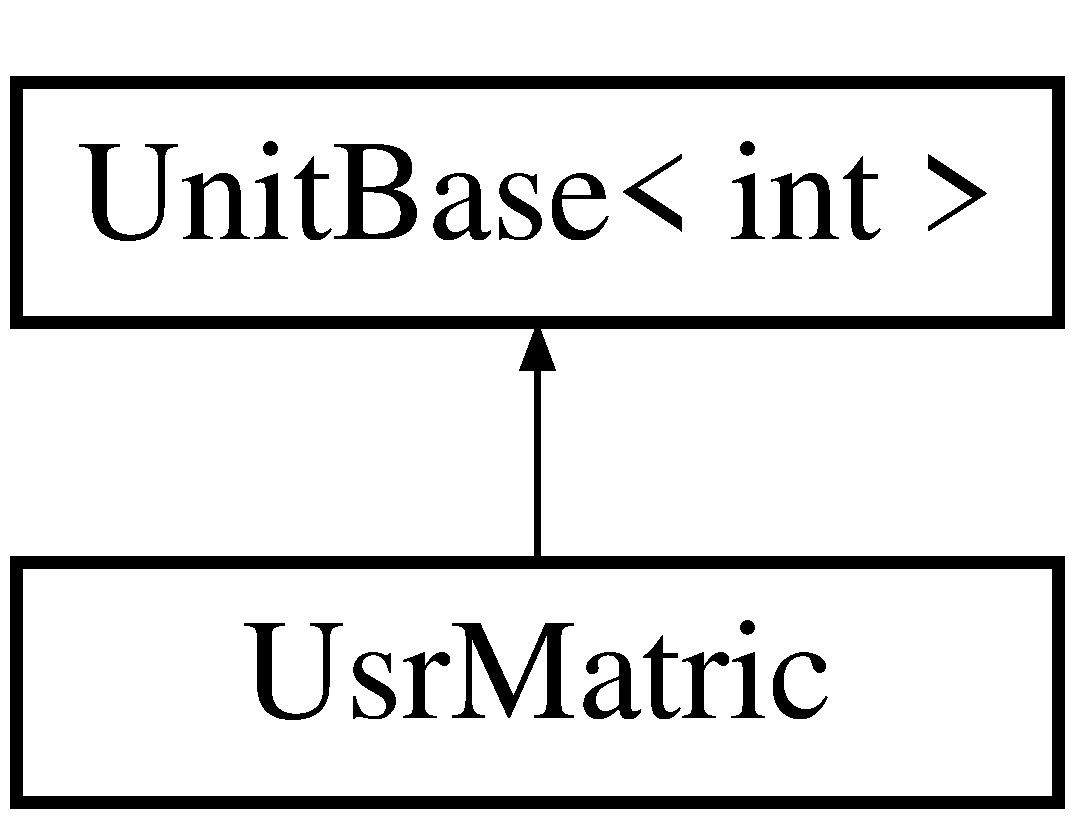
\includegraphics[height=2.000000cm]{classUsrMatric}
\end{center}
\end{figure}
\subsection*{Public Member Functions}
\begin{DoxyCompactItemize}
\item 
\hypertarget{classUsrMatric_acc7320dcfc8978fe9cc142340adb99c1}{{\bfseries Usr\-Matric} (const int \&)  throw (invalid\-\_\-argument)}\label{classUsrMatric_acc7320dcfc8978fe9cc142340adb99c1}

\end{DoxyCompactItemize}
\subsection*{Additional Inherited Members}


\subsection{Detailed Description}
Define a matrícula de um \hyperlink{classManager}{Manager}. 

Tem a função de identificar de forma única um \hyperlink{classManager}{Manager}, seja ele Administrador ou Gerente. 

The documentation for this class was generated from the following files\-:\begin{DoxyCompactItemize}
\item 
Base\-Unit.\-h\item 
Base\-Unit.\-cpp\end{DoxyCompactItemize}

\hypertarget{classUsrName}{\section{Usr\-Name Class Reference}
\label{da/df7/classUsrName}\index{Usr\-Name@{Usr\-Name}}
}


Define o nome de um \hyperlink{classUser}{User} (\hyperlink{classCustomer}{Customer} ou \hyperlink{classManager}{Manager}).  




{\ttfamily \#include $<$Base\-Unit.\-h$>$}

Inheritance diagram for Usr\-Name\-:\begin{figure}[H]
\begin{center}
\leavevmode
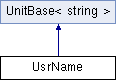
\includegraphics[height=2.000000cm]{da/df7/classUsrName}
\end{center}
\end{figure}
\subsection*{Public Member Functions}
\begin{DoxyCompactItemize}
\item 
\hyperlink{classUsrName_a0b0d5b9167309872d29c60a1946375af}{Usr\-Name} ()
\begin{DoxyCompactList}\small\item\em Construtor padrão de \hyperlink{classUsrName}{Usr\-Name}. \end{DoxyCompactList}\item 
\hyperlink{classUsrName_a3028672b21248ef880a01e3621e02827}{Usr\-Name} (const string \&)  throw (invalid\-\_\-argument)
\begin{DoxyCompactList}\small\item\em Construtor base de \hyperlink{classUsrName}{Usr\-Name}. \end{DoxyCompactList}\end{DoxyCompactItemize}
\subsection*{Additional Inherited Members}


\subsection{Detailed Description}
Define o nome de um \hyperlink{classUser}{User} (\hyperlink{classCustomer}{Customer} ou \hyperlink{classManager}{Manager}). 

Este tipo serve para regular o login de usuários em geral. 

\subsection{Constructor \& Destructor Documentation}
\hypertarget{classUsrName_a0b0d5b9167309872d29c60a1946375af}{\index{Usr\-Name@{Usr\-Name}!Usr\-Name@{Usr\-Name}}
\index{Usr\-Name@{Usr\-Name}!UsrName@{Usr\-Name}}
\subsubsection[{Usr\-Name}]{\setlength{\rightskip}{0pt plus 5cm}Usr\-Name\-::\-Usr\-Name (
\begin{DoxyParamCaption}
{}
\end{DoxyParamCaption}
)}}\label{da/df7/classUsrName_a0b0d5b9167309872d29c60a1946375af}


Construtor padrão de \hyperlink{classUsrName}{Usr\-Name}. 

Define a string vazia como valor de não-\/inicialização deste tipo básico \hypertarget{classUsrName_a3028672b21248ef880a01e3621e02827}{\index{Usr\-Name@{Usr\-Name}!Usr\-Name@{Usr\-Name}}
\index{Usr\-Name@{Usr\-Name}!UsrName@{Usr\-Name}}
\subsubsection[{Usr\-Name}]{\setlength{\rightskip}{0pt plus 5cm}Usr\-Name\-::\-Usr\-Name (
\begin{DoxyParamCaption}
\item[{const string \&}]{name}
\end{DoxyParamCaption}
)  throw (invalid\-\_\-argument)}}\label{da/df7/classUsrName_a3028672b21248ef880a01e3621e02827}


Construtor base de \hyperlink{classUsrName}{Usr\-Name}. 

É preferível que se utilize este construtor, pois ele já faz a validação automática do valor a ser definido. 

The documentation for this class was generated from the following files\-:\begin{DoxyCompactItemize}
\item 
Base\-Unit.\-h\item 
Base\-Unit.\-cpp\end{DoxyCompactItemize}

\hypertarget{classUsrPassword}{\section{Usr\-Password Class Reference}
\label{classUsrPassword}\index{Usr\-Password@{Usr\-Password}}
}


Define a senha de um \hyperlink{classUser}{User} (Customer ou \hyperlink{classManager}{Manager}).  




{\ttfamily \#include $<$Base\-Unit.\-h$>$}

Inheritance diagram for Usr\-Password\-:\begin{figure}[H]
\begin{center}
\leavevmode
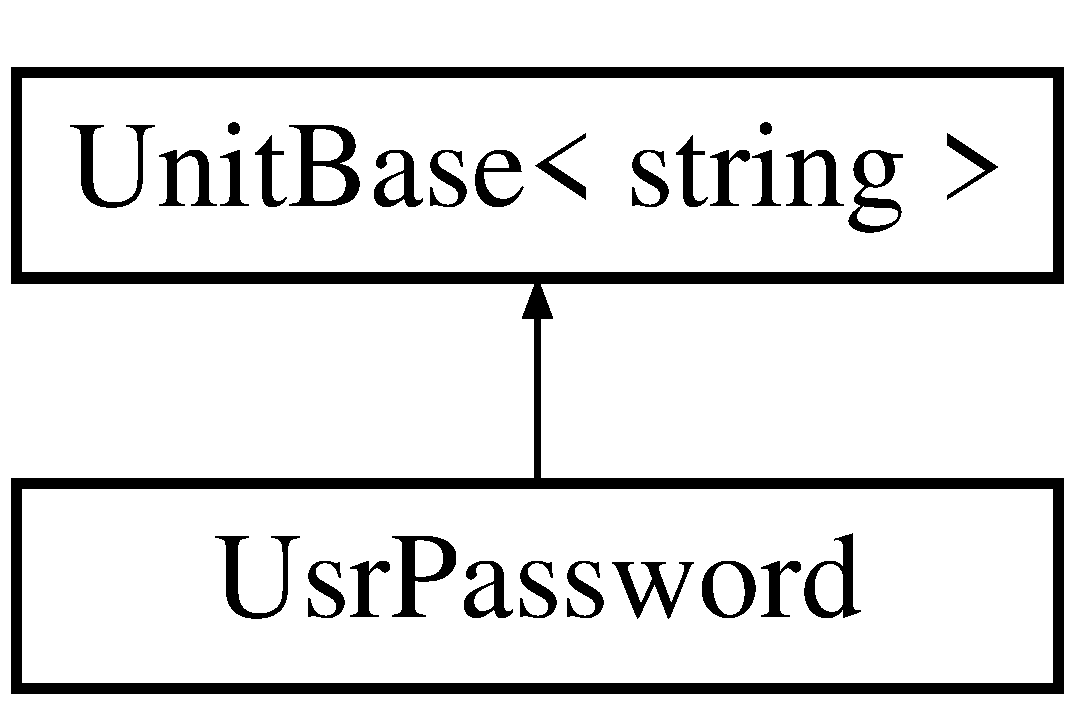
\includegraphics[height=2.000000cm]{classUsrPassword}
\end{center}
\end{figure}
\subsection*{Public Member Functions}
\begin{DoxyCompactItemize}
\item 
\hypertarget{classUsrPassword_ab99c93719778f9560712675b1febb3cb}{{\bfseries Usr\-Password} (const string \&)  throw (invalid\-\_\-argument)}\label{classUsrPassword_ab99c93719778f9560712675b1febb3cb}

\end{DoxyCompactItemize}
\subsection*{Additional Inherited Members}


\subsection{Detailed Description}
Define a senha de um \hyperlink{classUser}{User} (Customer ou \hyperlink{classManager}{Manager}). 

Este tipo básico tem a função de controlar o login de usuários em geral. 

The documentation for this class was generated from the following files\-:\begin{DoxyCompactItemize}
\item 
Base\-Unit.\-h\item 
Base\-Unit.\-cpp\end{DoxyCompactItemize}

\hypertarget{classUsrType}{\subsection{Usr\-Type Class Reference}
\label{d1/dd4/classUsrType}\index{Usr\-Type@{Usr\-Type}}
}


Codifica tipos de conta.  




{\ttfamily \#include $<$Base\-Unit.\-h$>$}

Inheritance diagram for Usr\-Type\-:\begin{figure}[H]
\begin{center}
\leavevmode
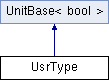
\includegraphics[height=2.000000cm]{d1/dd4/classUsrType}
\end{center}
\end{figure}
\subsubsection*{Public Member Functions}
\begin{DoxyCompactItemize}
\item 
\hyperlink{classUsrType_a51a73c6f2cfbca3174120a2796957c03}{Usr\-Type} ()
\begin{DoxyCompactList}\small\item\em Construtor padrão de \hyperlink{classUsrType}{Usr\-Type}. \end{DoxyCompactList}\item 
\hyperlink{classUsrType_a774f3a391ac5741802862cb7de682bb9}{Usr\-Type} (const bool \&)  throw (invalid\-\_\-argument)
\begin{DoxyCompactList}\small\item\em Construtor base de \hyperlink{classUsrType}{Usr\-Type}. \end{DoxyCompactList}\end{DoxyCompactItemize}
\subsubsection*{Additional Inherited Members}


\subsubsection{Detailed Description}
Codifica tipos de conta. 

Possui duas utilizações\-: Acc\-Type\-: Codifica tipos de conta (Normal / Especial) Man\-Type\-: Codifica tipos de manager (Gerente / Administrador) 

Definition at line 120 of file Base\-Unit.\-h.



\subsubsection{Constructor \& Destructor Documentation}
\hypertarget{classUsrType_a51a73c6f2cfbca3174120a2796957c03}{\index{Usr\-Type@{Usr\-Type}!Usr\-Type@{Usr\-Type}}
\index{Usr\-Type@{Usr\-Type}!UsrType@{Usr\-Type}}
\paragraph[{Usr\-Type}]{\setlength{\rightskip}{0pt plus 5cm}Usr\-Type\-::\-Usr\-Type (
\begin{DoxyParamCaption}
{}
\end{DoxyParamCaption}
)}}\label{d1/dd4/classUsrType_a51a73c6f2cfbca3174120a2796957c03}


Construtor padrão de \hyperlink{classUsrType}{Usr\-Type}. 

Define o valor N\-O\-R\-M\-A\-L/\-G\-E\-R\-E\-N\-T\-E como valor de não-\/inicialização deste tipo básico. 

Definition at line 90 of file Base\-Unit.\-cpp.

\hypertarget{classUsrType_a774f3a391ac5741802862cb7de682bb9}{\index{Usr\-Type@{Usr\-Type}!Usr\-Type@{Usr\-Type}}
\index{Usr\-Type@{Usr\-Type}!UsrType@{Usr\-Type}}
\paragraph[{Usr\-Type}]{\setlength{\rightskip}{0pt plus 5cm}Usr\-Type\-::\-Usr\-Type (
\begin{DoxyParamCaption}
\item[{const bool \&}]{usr\-Type}
\end{DoxyParamCaption}
)  throw (invalid\-\_\-argument)}}\label{d1/dd4/classUsrType_a774f3a391ac5741802862cb7de682bb9}


Construtor base de \hyperlink{classUsrType}{Usr\-Type}. 

É preferível que se utilize este construtor, pois ele já faz a validação automática do valor a ser definido. 

Definition at line 95 of file Base\-Unit.\-cpp.



The documentation for this class was generated from the following files\-:\begin{DoxyCompactItemize}
\item 
Base\-Unit.\-h\item 
Base\-Unit.\-cpp\end{DoxyCompactItemize}

\addcontentsline{toc}{part}{Index}
\printindex
\end{document}
